\documentclass{beamer}\usepackage[]{graphicx}\usepackage[]{color}
%% maxwidth is the original width if it is less than linewidth
%% otherwise use linewidth (to make sure the graphics do not exceed the margin)
\makeatletter
\def\maxwidth{ %
  \ifdim\Gin@nat@width>\linewidth
    \linewidth
  \else
    \Gin@nat@width
  \fi
}
\makeatother

\definecolor{fgcolor}{rgb}{0.345, 0.345, 0.345}
\newcommand{\hlnum}[1]{\textcolor[rgb]{0.686,0.059,0.569}{#1}}%
\newcommand{\hlstr}[1]{\textcolor[rgb]{0.192,0.494,0.8}{#1}}%
\newcommand{\hlcom}[1]{\textcolor[rgb]{0.678,0.584,0.686}{\textit{#1}}}%
\newcommand{\hlopt}[1]{\textcolor[rgb]{0,0,0}{#1}}%
\newcommand{\hlstd}[1]{\textcolor[rgb]{0.345,0.345,0.345}{#1}}%
\newcommand{\hlkwa}[1]{\textcolor[rgb]{0.161,0.373,0.58}{\textbf{#1}}}%
\newcommand{\hlkwb}[1]{\textcolor[rgb]{0.69,0.353,0.396}{#1}}%
\newcommand{\hlkwc}[1]{\textcolor[rgb]{0.333,0.667,0.333}{#1}}%
\newcommand{\hlkwd}[1]{\textcolor[rgb]{0.737,0.353,0.396}{\textbf{#1}}}%

\usepackage{framed}
\makeatletter
\newenvironment{kframe}{%
 \def\at@end@of@kframe{}%
 \ifinner\ifhmode%
  \def\at@end@of@kframe{\end{minipage}}%
  \begin{minipage}{\columnwidth}%
 \fi\fi%
 \def\FrameCommand##1{\hskip\@totalleftmargin \hskip-\fboxsep
 \colorbox{shadecolor}{##1}\hskip-\fboxsep
     % There is no \\@totalrightmargin, so:
     \hskip-\linewidth \hskip-\@totalleftmargin \hskip\columnwidth}%
 \MakeFramed {\advance\hsize-\width
   \@totalleftmargin\z@ \linewidth\hsize
   \@setminipage}}%
 {\par\unskip\endMakeFramed%
 \at@end@of@kframe}
\makeatother

\definecolor{shadecolor}{rgb}{.97, .97, .97}
\definecolor{messagecolor}{rgb}{0, 0, 0}
\definecolor{warningcolor}{rgb}{1, 0, 1}
\definecolor{errorcolor}{rgb}{1, 0, 0}
\newenvironment{knitrout}{}{} % an empty environment to be redefined in TeX

\usepackage{alltt}% usefull options [handout]
\usepackage{graphicx}
\usepackage{amsmath}
\usepackage{hyperref}

%%% EU logo
% small version for upper right corner of normal pages
\pgfdeclareimage[width=12.8cm]{jrc-logo}{JRC_header}
\logo{\pgfuseimage{jrc-logo}}
\pgfdeclareimage[height=5.5mm]{footimage}{JRC_footer}
\pgfdeclareimage[width=0.5\textwidth]{title-image}{Bayer}
\titlegraphic{\pgfuseimage{title-image}}
%%% end EU logo


% NOTE: 1cm = 0.393 in = 28.346 pt;    1 pt = 1/72 in = 0.0352 cm
\setbeamersize{text margin right=3.5mm, text margin left=7.5mm}  % text margin

% colors to be used
\definecolor{text-grey}{rgb}{0.45, 0.45, 0.45} % grey text on white background
\definecolor{bg-grey}{rgb}{0.66, 0.65, 0.60} % grey background (for white text)
\definecolor{eu-blue}{RGB}{55, 172, 222} % blue text
\definecolor{drk-blue}{RGB}{0, 51, 102} % blue text
\definecolor{fu-blue}{RGB}{0, 51, 102} % blue text
\definecolor{fu-green}{RGB}{153, 204, 0} % green text
\definecolor{fu-red}{RGB}{204, 0, 0} % red text (used by \alert)

% switch off the sidebars
\setbeamersize{sidebar width left=0cm, sidebar width right=0mm}
\setbeamertemplate{sidebar right}{}
\setbeamertemplate{sidebar left}{}
\setbeamertemplate{navigation symbols}{}%remove navigation symbols

% frame title
\setbeamertemplate{frametitle}{%
    \vskip-5pt \color{drk-blue}\Large%
    \begin{minipage}[b][23pt]{\textwidth}%
    \flushleft \textbf{\insertframetitle}%
    \end{minipage}%
}

%%% title page
\setbeamertemplate{title page}{
% set the title
\parbox[top][2.8cm][c]{\textwidth}{\begin{center} \color{drk-blue}\LARGE \textbf{\inserttitle}  \\ \vspace{10pt} \small \insertsubtitle \end{center}}

% title image of the presentation
\begin{minipage}{0.5\textwidth}
\flushleft
%\hspace{-7.5mm}
\inserttitlegraphic
\end{minipage}
% Author info
\hspace{0.5cm}
\begin{minipage}{0.4\textwidth}
{\flushleft \color{drk-blue} \textbf{\insertauthor} \\ \insertinstitute }
\end{minipage}
}
%%% end title page

%%% colors
\usecolortheme{lily}
\setbeamercolor*{normal text}{fg=drk-blue, bg=white}
\setbeamercolor*{alerted text}{fg=fu-red}
\setbeamercolor*{example text}{fg=fu-green}
\setbeamercolor*{structure}{fg=fu-blue}

\setbeamercolor*{block title}{fg=white,bg=black!50}
\setbeamercolor*{block title alerted}{fg=white,bg=black!50}
\setbeamercolor*{block title example}{fg=white,bg=black!50}

\setbeamercolor*{block body}{bg=black!10}
\setbeamercolor*{block body alerted}{bg=black!10}
\setbeamercolor*{block body example}{bg=black!10}

\setbeamercolor{item}{fg=drk-blue}
%%% end colors

\setbeamertemplate{itemize items}[circle] % if you want a ball
\setbeamertemplate{itemize subitem}[circle] % if you wnat a circle
\setbeamertemplate{itemize subsubitem}[circle] % if you want a triangle

%%% headline
\setbeamertemplate{headline}{
\insertlogo
}
%%% end headline

%%% footline
\newcommand{\footlinetext}{\insertdate}
\setbeamertemplate{footline}{
\begin{minipage}{58mm}
 \color{drk-blue} \hspace{7.5mm} %European Commission
\end{minipage}
\hspace{0.1mm} 
\begin{minipage}{8.5mm}
 \pgfuseimage{footimage}
\end{minipage}
\hspace{0.1mm}
\begin{minipage}{50mm}
 \color{drk-blue} 
 \flushright \insertframenumber \,/\,\inserttotalframenumber
\end{minipage}
}
%%% end footline

%%% code to remove headline
\makeatletter
    \newenvironment{withoutheadline}{
        \setbeamertemplate{headline}[default]
        \def\beamer@entrycode{\vspace*{-\headheight}}
    }{}
\makeatother
%%% end code to remove headline
    % THIS is the line that includes the EU template!
\usepackage{arev,t1enc}
\usepackage[T1]{fontenc}
\fontfamily{verdana}\selectfont
\usepackage{tikz}
\usetikzlibrary{shapes,arrows}
\usepackage{amsmath,bm,times}
\newcommand{\mx}[1]{\mathbf{\bm{#1}}} % Matrix command
\newcommand{\vc}[1]{\mathbf{\bm{#1}}} % Vector command


%\titleimage{JRC} % pdf or png
\title{Assessment For All (a4a)}
\subtitle{The stock assessment model}
\author{The a4a team}
\institute[JRC]{European Commission\\ Joint Research Centre}
\date{August 2014}
\subject{Fisheries Management}
\IfFileExists{upquote.sty}{\usepackage{upquote}}{}

\begin{document}

\section{setup} % load libraries and data, set up knitr




%*******************************************
\begin{frame}%[plain]
\titlepage
	\begin{flushright}
		
\includegraphics[width=0.1\textwidth]{cc.png}
	\end{flushright}
\end{frame}

\section{Stock assessment model details}

\newcommand{\E}[1]{\text{E}\left[#1\right]}
\newcommand{\Var}[1]{\text{Var}\left[#1\right]}

%*******************************************
\begin{frame}{The a4a stock assessment framework}

The a4a stock assessment framework is a statistical catch-at-age model written in R with ADMB underneath (to find the parameters).

It was written with the aim of quickly developing stock assessment models for stocks with limited time series. 

\end{frame}

\begin{frame}{The a4a stock assessment framework}

A model is defined by submodels, which specify the different parts of a statistical catch-at-age model.

There are 5 submodels in operation: 
\begin{itemize}
  \item a model for F-at-age
  \item a model for the initial age structure
  \item a model for recruitment
  \item a (list) of model(s) for abundance indices catchability-at-age
  \item a list of models for the observation variance of catch-at-age and abundance indices.
\end{itemize}

\end{frame}

\begin{frame}{The a4a stock assessment framework}

The submodels form use linear models. This opens the possibility of using the linear modelling tools available in R: see for example the \href{http://cran.r-project.org/web/packages/mgcv/index.html}{mgcv} gam formulas, or factorial design formulas using lm(). In R's linear modelling language, a constant model is coded as $\sim 1$, while a slope over age would simply be $\sim age$. For example, we can write a traditional year/age separable F model like $\sim factor(age) + factor(year)$.

\end{frame}

\begin{frame}{linear model examples}

\begin{knitrout}
\definecolor{shadecolor}{rgb}{0.969, 0.969, 0.969}\color{fgcolor}\begin{kframe}
\begin{alltt}
\hlstd{rec} \hlkwb{<-} \hlkwd{c}\hlstd{(}\hlkwd{rec}\hlstd{(ple4))}
\hlstd{year} \hlkwb{<-} \hlkwd{as.numeric}\hlstd{(}\hlkwd{dimnames}\hlstd{(}\hlkwd{rec}\hlstd{(ple4))[[}\hlnum{2}\hlstd{]])}
\hlstd{rlm} \hlkwb{<-} \hlkwd{lm}\hlstd{(rec} \hlopt{~} \hlstd{year)}
\hlstd{scafit} \hlkwb{<-} \hlkwd{sca}\hlstd{(ple4, ple4.indices,} \hlkwc{srmodel} \hlstd{=} \hlopt{~}\hlstd{year)}
\end{alltt}
\end{kframe}
\end{knitrout}


\end{frame}

\begin{frame}{linear model examples}

\begin{knitrout}
\definecolor{shadecolor}{rgb}{0.969, 0.969, 0.969}\color{fgcolor}\begin{figure}[]

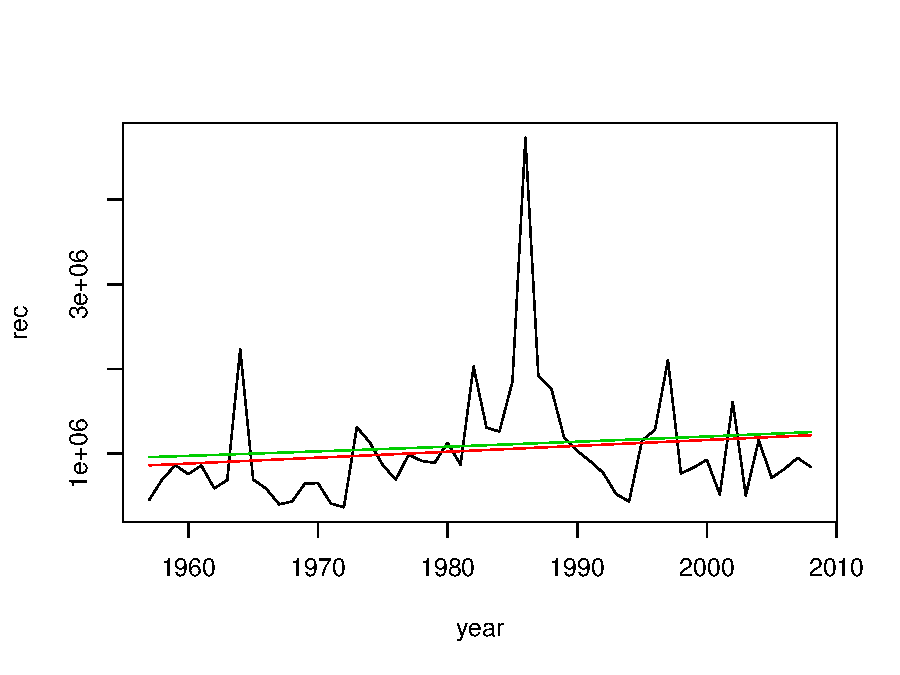
\includegraphics[width=\maxwidth]{figure/unnamed-chunk-2} \caption[Linear model for recruitment]{Linear model for recruitment\label{fig:unnamed-chunk-2}}
\end{figure}


\end{knitrout}


\end{frame}

\begin{frame}{linear model examples}

\begin{knitrout}
\definecolor{shadecolor}{rgb}{0.969, 0.969, 0.969}\color{fgcolor}\begin{kframe}
\begin{alltt}
\hlstd{rlm} \hlkwb{<-} \hlkwd{lm}\hlstd{(rec} \hlopt{~} \hlkwd{factor}\hlstd{(year))}
\hlstd{scafit} \hlkwb{<-} \hlkwd{sca}\hlstd{(ple4, ple4.indices,} \hlkwc{srmodel} \hlstd{=} \hlopt{~}\hlkwd{factor}\hlstd{(year))}
\end{alltt}
\end{kframe}
\end{knitrout}


\end{frame}

\begin{frame}{linear model examples}

\begin{knitrout}
\definecolor{shadecolor}{rgb}{0.969, 0.969, 0.969}\color{fgcolor}\begin{figure}[]

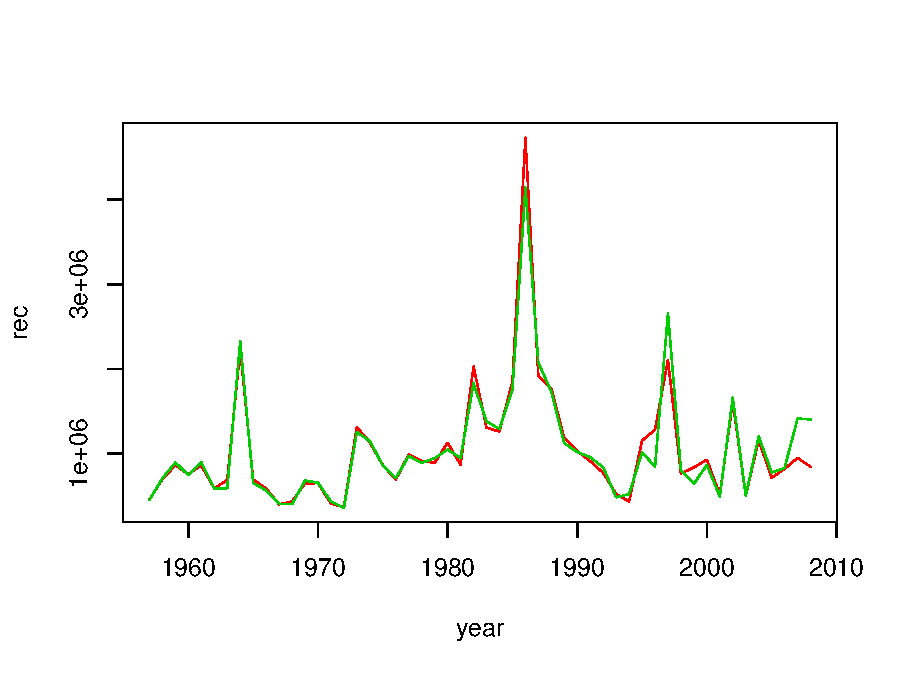
\includegraphics[width=\maxwidth]{figure/unnamed-chunk-4} \caption[Linear model for recruitment]{Linear model for recruitment\label{fig:unnamed-chunk-4}}
\end{figure}


\end{knitrout}


\end{frame}

%\begin{frame}{linear model examples}
%
%<<echo=TRUE>>=
%rlm <- lm(rec~year + I(year^2) + I(year^3) + I(year^4))
%scafit <- sca(ple4, ple4.indices, srmodel=~year + I(year^2) + I(year^3) + I(year^4))
%@
%
%\end{frame}
%
%\begin{frame}{linear model examples}
%
%<<fig.cap='Linear model for recruitment'>>=
%plot(rec~year, type='l')
%lines(predict(rlm)~year, col=2)
%lines(c(stock.n(scafit)[1])~year, col=3)
%@
%
%\end{frame}

\begin{frame}{Model detail}

\begin{equation*}
e^{\E{\log C}} = \frac{\color{red}F}{{\color{red}F}+M}\left(1 - e^{-{\color{red}F}-M}\right) {\color{red}R}e^{-\sum {\color{red}F} + M}
\end{equation*}

and

\begin{equation*}
e^{\E{\log I}} = {\color{red}Q} {\color{red}R}e^{-\sum {\color{red}F} + M}
\end{equation*}

and

\begin{equation*}
\Var{\log C_{ay}} = {\color{red}\sigma^2_{ay}} \qquad \Var{\log I_{ays}} = {\color{red}\tau^2_{ays}}
\end{equation*}

\end{frame} 

\begin{frame}{Model detail}

linear models for
\begin{itemize}
  \item log F
  \item log Q
  \item log observation variances
  \item log initial age structure  
\end{itemize}

Recruitment is modelled as a \alert{fixed variance} random effect with linear models for
\begin{itemize}
  \item log a
  \item log b
\end{itemize}
where relevant.  Models available: Ricker, Beverton Holt, smooth hockeystick, geometric mean
\end{frame} 

\begin{frame}{Linear models}

It is not always obvious that stock assessments are often composed of linear models.

For example, the classical separable F assumption is simply that
\begin{align*}
F_{ay} = S_a \times F_y 
\end{align*}
which, in linear modelling parlance is
\begin{align*}
\log F \sim \text{age} + \text{year} 
\end{align*}

\end{frame}

\begin{frame}{Intuitive Modelling}

The "language" of linear models has been developing within the statistical community for many years:

  \begin{itemize}
  \item 1965 J. A. Nelder, notation for randomized block design
  \item 1973 Wilkinson and Rodgers, symbolic description for factorial designs
  \item 1990 Hastie and Tibshirani, introduced notation for smoothers
  \item 1991 Chambers and Hastie, further developed for use in S
  \end{itemize}

Many modelling software use this language:  Minitab, spss, genstat, SAS, R, S-plus.

\end{frame}


\begin{frame}{Some examples}
A separable model where the level of F is smooth through time

\begin{align*}
  \log F \sim \text{age} + \text{s(year)}
\end{align*}
\end{frame}


\begin{frame}{Some examples}
A separable model where F is smooth over age

\begin{align*}
  \log F \sim \text{s(age)} + \text{year}
\end{align*}
\end{frame}


\begin{frame}{Some examples}
F is smooth over age and year

\begin{align*}
  \log F \sim \text{s(age, year)}
\end{align*}
\end{frame}

\section{Future directions} % A little bit on model selection

% We need layers to draw the block diagram
\pgfdeclarelayer{background}
\pgfdeclarelayer{foreground}
\pgfsetlayers{background,main,foreground}

% Define a few styles and constants
\tikzstyle{model}=[draw, fill=blue!20, text width=5em, text centered, minimum height=2.5em]
\tikzstyle{modelsels} = [model, text width=6em, fill=red!20, minimum height=12em, rounded corners]
\def\blockdist{2.3}
\def\edgedist{2.5}

% The assessment process
\begin{frame}{An Assessment Process}
\begin{center}
\begin{tikzpicture}
    % draw the blocks
    \node (modsel) [modelsels] {Model Selection};
    \path (modsel.140)+(-\blockdist,0) node (mod1) [model] {Model 1};
    \path (modsel.-150)+(-\blockdist,0) node (mod2) [model] {Model 2};
    
    % draw the arrows and text
    \path [draw, ->] (mod1) -- (modsel.west |- mod1) ;
    \path [draw, ->] (mod2) -- (modsel.west |- mod2);
    \node (choices) [below of=mod2] {Scenarios};
    \path (modsel.south west)+(-0.6,-0.6) node (assess) {Assessment};
    \draw [->] (modsel.0) -- (\edgedist,0) node[right] {Advice};
    
   % draw the box around the models
    \begin{pgfonlayer}{background}
        % Compute a few helper coordinates
        \path (mod1.west |- modsel.north)+(-0.5,0.3) node (a) {};
        \path (assess.south -| modsel.east)+(+0.3,-0.2) node (b) {};
        \path[fill=yellow!20,rounded corners, draw=black!50, dashed] (a) rectangle (b);
        \path (mod1.north west)+(-0.2,0.2) node (a) {};
        \path (choices.south -| mod1.east)+(+0.2,-0.2) node (b) {};
        \path[fill=blue!10,rounded corners, draw=black!50, dashed] (a) rectangle (b);
    \end{pgfonlayer}
\end{tikzpicture}
\end{center}
\end{frame}

\begin{frame}{Model Averaging can help automation}
\begin{center}
\begin{tikzpicture}
    % draw the blocks
    \node (modsel) [modelsels] {Model Averaging};
    \path (modsel.140)+(-\blockdist,0) node (mod1) [model] {Model 1};
    \path (modsel.-150)+(-\blockdist,0) node (mod2) [model] {Model 2};
    
    % draw the arrows and text
    \path [draw, ->] (mod1) -- (modsel.west |- mod1) ;
    \path [draw, ->] (mod2) -- (modsel.west |- mod2);
    \node (choices) [below of=mod2] {Scenarios};
    \path (choices.south)+(0,-0.6) node (assess) {Assessment};
    \draw [->] (modsel.0) -- (\edgedist,0) node[right] {Advice};
    
   % draw the box around the models
    \begin{pgfonlayer}{background}
        % Compute a few helper coordinates
        \path (mod1.north west)+(-0.5,0.5) node (a) {};
        \path (assess.south -| choices.east)+(+0.5,-0.2) node (b) {};
        \path[fill=yellow!20,rounded corners, draw=black!50, dashed] (a) rectangle (b);
        \path (mod1.north west)+(-0.2,0.2) node (a) {};
        \path (choices.south -| mod1.east)+(+0.2,-0.2) node (b) {};
        \path[fill=blue!10,rounded corners, draw=black!50, dashed] (a) rectangle (b);
    \end{pgfonlayer}
\end{tikzpicture}
\end{center}
\end{frame}

\begin{frame}{Expert knowledge for model specification}

Different plausible models for different levels
\begin{itemize}
\item Management area level (North Sea, Baltic Sea, ...)
\item Species type (roundfish, flatfish, pelagic, Nephrops)
\item specific groups (North Sea gadoids)
\end{itemize}

\vspace{5mm}
This provides a framework for setting up plausible models for new species.

\vspace{5mm}
Can lots of simple models averaged = a good model?

\emph{Kearns: Can a set of weak learners create a single strong learner}

\end{frame}

\begin{frame}{}

\begin{center}
\Large\textbf{Thank you for listening!}
\end{center}

\end{frame}

\begin{frame}{What we can do, what we can't do}

Can:
\begin{itemize}
\item missing values: missing at random
\item multiple surveys
\item variable Q, F, variance
\item splines (fixed degreed of freedom)
\item stock recruit relationship (fixed variance)
\item stock recruit relationship (estimated variance) SLOW
\item \emph{fixed variance random effects: RW1, RW2, seasonal, user specified}
\end{itemize}

Can't:
\begin{itemize}
\item estimate random effect variance
\item estimate smoothing parameters
\item estimate growth parameters
\end{itemize}

\end{frame}

\begin{frame}{What we can do}

\begin{itemize}
\item simulate from the distribution of model params
\begin{itemize}
\item normal approx
\item avoids the need for delta approx
\item can be biased, but we can also use MCMC if desired
\end{itemize}
\item we can approximate the (joint) distribution of
\begin{itemize}
\item terminal year Fs and Ns
\item terminal year Fbar and Fmsy
\item F / Fmsy
\end{itemize}
\end{itemize}

\end{frame}


\end{document}
